\chapter{Система за автоматизирано отдалечено управление на РОБКО 01 с
възможност за ръчен контрол}
%използвани технологии
\section{Функционални изисквания}
Към настоящата разработка са поставени следните изисквания:
\begin{itemize}
    \item ръчно управление на РОБКО 01
    \item управление на робота чрез текстови команди
    \item подаване на команди през интернет
    \item четене на команди от файл
    \item опашка за команди
    \item едновременно движение на всички мотори
    \item засичане на предмет в щипката на робота
\end{itemize}
\section{Топология на системата}
На фигура \ref{fig:system} е показана блокова схема на проектираната система. Жълтите стрелки обозначават информационни сигнали, а кафявите - захранващи напрежения и токове.\\
\indent{}
Основната платка реализира връзките между отделните компоненти на системата. Прякото управление на робота се извършва от микроконтролер STM32L476RG, разположен на собствена платка. Микроконтролерът получава информация относно какви движения трябва да изпълни роботът от два източника: два джойстика (ръчно управление) и компютър в интернет, наричан клиент. Клиентът изпраща команди през интернет до втори компютър - сървъра. Сървърът е свързан с микроконтролера и препраща командите към него.\\
\indent{}
\begin{figure}[!htbp]
    \centering
    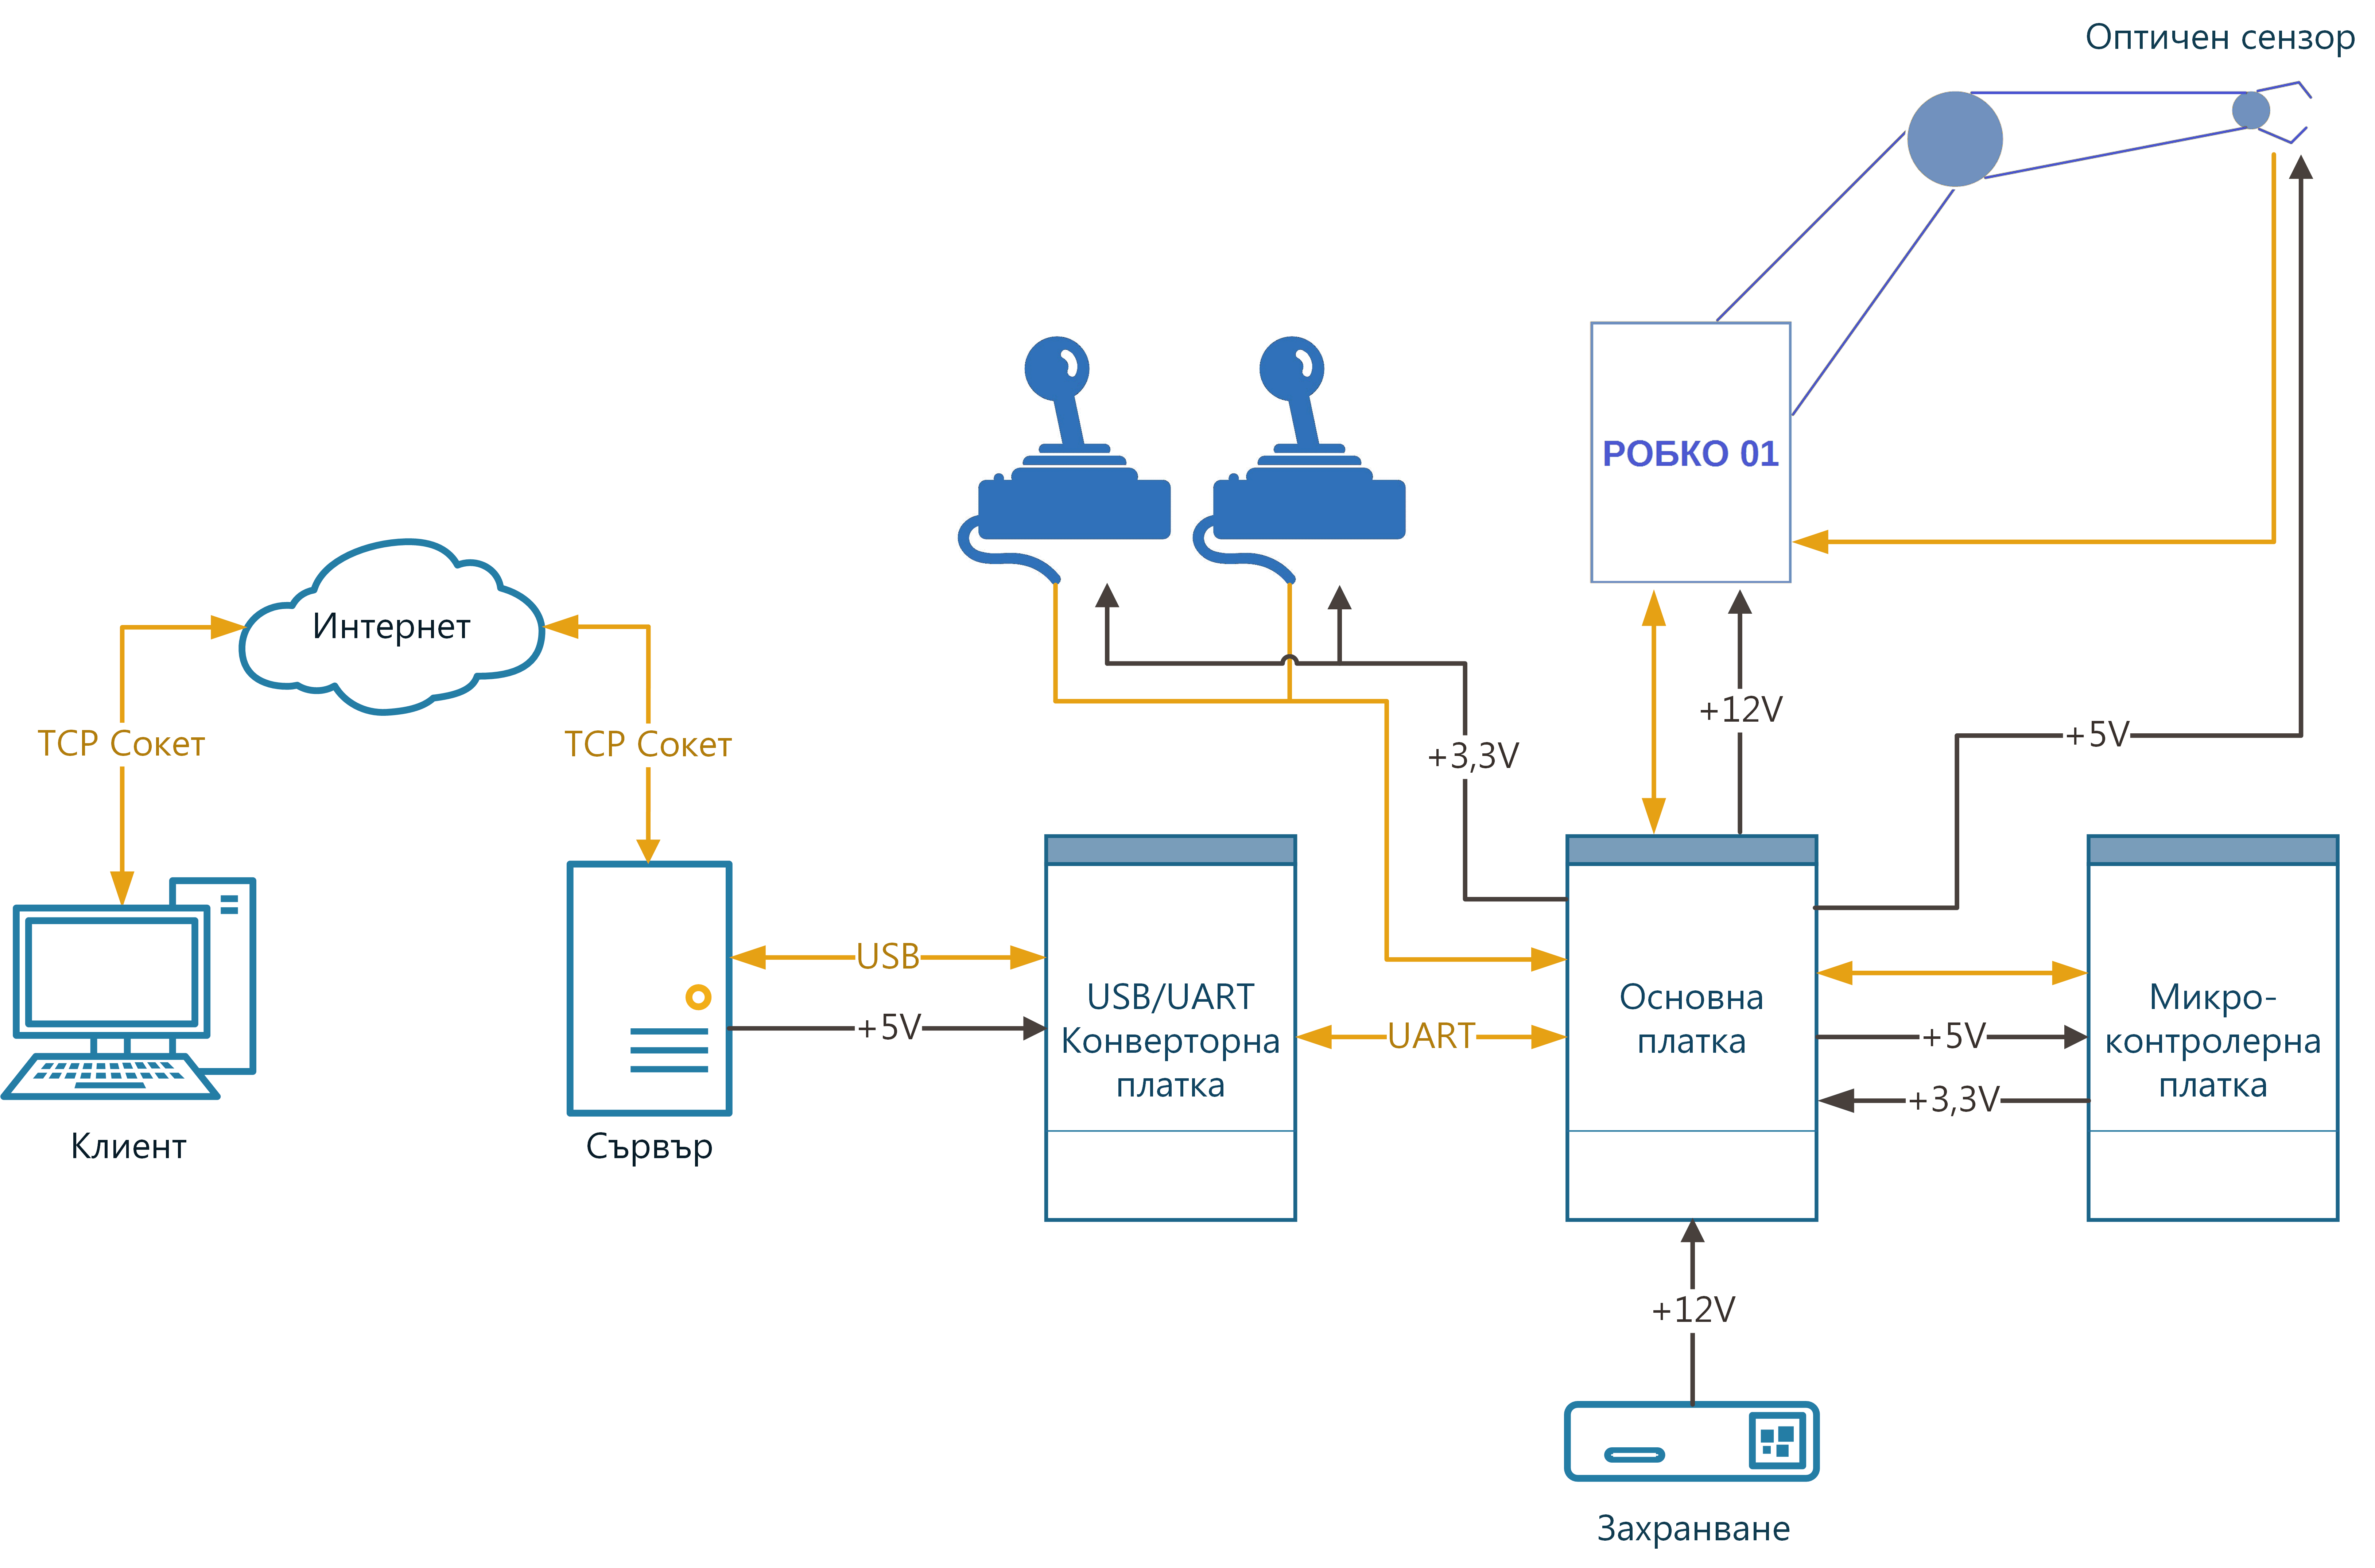
\includegraphics[angle=90,origin=center,width=\linewidth]{pictures/robko_system_diagram.png}
    \caption{Блокова схема на системата}
    \label{fig:system}
\end{figure}
\section{Компоненти на системата}
\subsection{РОБКО 01}
\subsubsection{Механика}
\indent{}
РОБКО 01 е антропоиден робот със шест степени на свобода, реализирани с кинематични връзки.
\cite{robko-man}
Изграден е от неподвижна основа, три звена и хващач. Задвижва се от шест стъпкови електромотора, означени с 5 на фигура \ref{fig:mech}. Те са монтирани от външната страна на първото звено(1). Във вътрешността му се помещават шест зъбни редуктора(6). Движението на моторите се предава към звената и щипката(4) чрез метални въжета и ролки(7).\\
\indent{}
Първото звено се върти около ос, перпендикулярна на основата. Второто(2) и третото(3) звено, наричани съответно рамо и лакът, се накланят съответно напред-назад и нагоре-надолу. Хващачът се върти и накланя нагоре-надолу. Тези движения се реализират посредством диференциална зъбна предавка, разположена между третото звено и хващача. Тя се задвижва от два мотора. При съпосочно въртене на моторите хващачът се накланя в съответната посока. Когато двата мотора се въртят противопосочно, едната страна на хващача се накланя нагоре, а другата надолу. Резултатното движение е въртене.\\
\indent{}
Върху второто звено е монтиран прекъсвач, който се затваря когато металното въже, затварящо хващача, се обтегне достатъчно. Това позволява да се засича дали хващачът е стиснал предмет. Тази функционалност не се използва в текущата разработка заради голямата сила, нужна за да се затвори прекъсвача, и опасността въжето да се скъса.
\FloatBarrier
\begin{figure}[!htb]
    \centering
    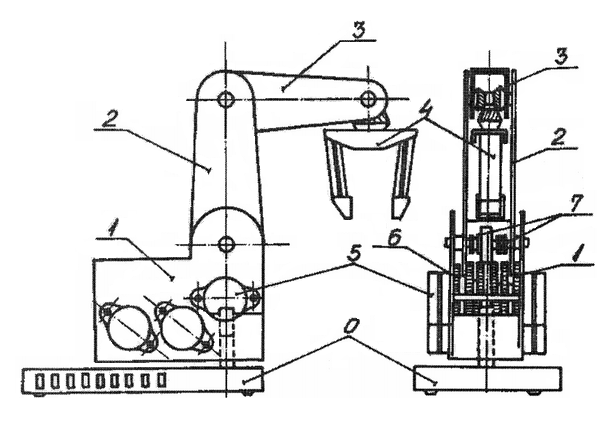
\includegraphics[width=\linewidth]{pictures/Robko_axis.PNG}
    \caption{РОБКО 01 - схема на механиката}
    \label{fig:mech}
\end{figure}
\subsubsection{Драйверна платка}
\indent{}
Драйверната платка на РОБКО 01 е описана подробно в ръководството за експлоатация
\cite{robko-man}, но липсват важни подробности. Не е обозначено кой сигнал на кой пин на конекторите е изведен. Липсват стойностите на пасивните елементи. Пропуснати са четири кондензатора. Не са дадени моделите на компонентите.\\
\indent{}
След анализ на печатната платка и с помощта на информация от интернет и от предишния собственик на робота, принципната електрическа схема на РОБКО 01 беше въстановена и попълнена с липсващата информация. На следващите страници е дадена въстановената принципна електрическа схема. Схемните страници от 10-та до 14-та включително са идентични на 9-та схемна страница и не са показани.

Цифровата логика на схемата е реализирана с ИС от серията 74LSxx и техни еквиваленти. Интегралните схеми се захранват от линеен регулатор на напрежение MA7805. На моторите и на регулатора се подава напрежение 12V.
\includepdf[pages={4},angle=90]{documents/schematic_bw.pdf}
\includepdf[pages={8-9},angle=90]{documents/schematic_bw.pdf}
\includepdf[pages={15-17},angle=90]{documents/schematic_bw.pdf}
Стъпковите електромотори са двуфазни униполярни. Двете фази са изградени от по две статорни намотки. Шестте мотора се управляват от транзисторни крайни стъпала с диодна защита от обратно напрежение. За всеки мотор отговаря по един 4-битов регистър, съхраняващ състоянията на намотките/фазите му. Чрез записване на данни в регистрите се контролира през кои намотки на стъпковите мотори да протича ток.\\
\indent{}
Не всяка от 16-те възможни стойности на регистрите съответства на позволено състояние на моторите. Непозволените комбинации се предотвратяват от логически елементи ИЛИ-НЕ. В таблица \ref{tab:step_order} са дадени позволените комбинации от токове през намотките на моторите. Индексите на токовете съответстват на индексите на битовете в регистрите за съответните мотори. За въртене в режим на полустъпка се изпълняват в дадения ред, а за режим на цяла стъпка се пропускат  полустъпките при които протича ток само през една намотка.
\begin{table}[!htb]
    \centering
    \begin{tabular}{|c|c|c|c|}
        \hline
        I$_0$ & I$_1$ & I$_2$ & I$_3$\\
        \hline
        1 & 0 & 0 & 0\\
        \hline
        1 & 0 & 1 & 0\\
        \hline
        0 & 0 & 1 & 0\\
        \hline
        0 & 1 & 1 & 0\\
        \hline
        0 & 1 & 0 & 0\\
        \hline
        0 & 1 & 0 & 1\\
        \hline
        0 & 0 & 0 & 1\\
        \hline
        1 & 0 & 0 & 1\\
        \hline
    \end{tabular}
    \captionsetup{width=0.65\linewidth}
    \caption{Поредност на стъпките на моторите за въртене в режим на полустъпка}
    \label{tab:step_order}
\end{table}
\captionsetup{width=\linewidth}
\\
\indent{}
Два допълнителни регистъра са заделени за осемте изходни пина на платката (OUT0-OUT7). Към изходите на тези регистри са свързани буфери с изходи от тип отворен колектор. Това позволява от изходните пинове на робота да се управляват товари, работещи на по-високо напрежение от ТТЛ интегралните схеми.\\
\indent{}
РОБКО 01 разполага и с осем входни пина (IN0-IN7). Данните от тях се буферират в повторители с високоимпедансно изходно състояние.

Достъпът до регистрите се контролира от 3-битов дешифратор, обуславящ 8 адреса. Първите шест адреса се отнасят за регистрите на стъпковите мотори. Последните два адреса отговарят едновременно за 8-те изходни пина и за 8-те входни пина.\\
\indent{}
Понеже РОБКО 01 е проектиран да се управлява от 8-битовия Правец 82, разполага с 8-битова
\footnote{Адресната магистрала на Правец 82 е 16-битова.
\cite{pravets82}
Разширителната платка, показана на фигура \ref{fig:orig_cntrl}, свързва РОБКО 01 с Правец 82 и транслира адресното пространство на робота в това на компютъра.}
адресна магистрала (A0-A7) и 8-битова магистрала за данни (D0-D7). Младшите
\footnote{При Правец 82 и РОБКО 01 нулевият бит е най-младши.}
4 бита от магистралата за данни се използват от компютъра (или микроконтролера) за да записва данни в регистрите на робота. Старшите четири бита се използват за четене на входните пинове на РОБКО 01.\\
\indent{}
С трите най-младши адресни бита се избира регистър или входящ буфер, а останалите адресни битове транслират тези адреси в адресното пространство на Правец 82. Те се свързват към логически елементи И-НЕ и ИЛИ-НЕ, които подават разрешаващ сигнал на дешифратора само ако старшите адресни битове имат правилните стойности. В таблица \ref{tab:addr_space} е описано адресното пространство на РОБКО 01. За права посока се приема реда на стъпки даден в таблица \ref{tab:step_order}, изпълняван от горе надолу.\\
\begin{table}[!htb]
    \centering
    \begin{tabular}{|c|c|c|}
        \hline
        Адрес & Мотор / буфер & Движение в права посока\\
        \hline
        0x98 & 0 - Ос на основата & Въртене наляво\\
        0x99 & 1 - Раменна става & Накланяне напред\\
        0x9A & 2 - Лакътна става & Повдигане нагоре\\
        0x9B & 3 - Щипка - диф. предавка, десен & Накланяне надолу\\
        0x9C & 4 - Щипка - диф. предавка, ляв & Накланяне нагоре\\
        0x9D & 5 - Щипка - пръсти & Отваряне\\
        \cline{3-3}
        0x9E & Младши входни/изходни битове & \multicolumn{1}{c}{}\\
        0x9F & Старши входни/изходни битове & \multicolumn{1}{c}{}\\
        \cline{1-2}
    \end{tabular}
    \caption{Адресно пространство на РОБКО 01}
    \label{tab:addr_space}
\end{table}
\indent{}
\FloatBarrier
РОБКО 01 има четири контролни сигнала - \textoverline{BS}, \textoverline{DINE}, \textoverline{I/O R} и \textoverline{I/O W}. Първите два не се използват.\\
\indent{}
\textoverline{I/O R} е разрешаващ сигнал за четене. Когато е в активно ниско ниво, входящите буфери подават на D4-D7 състоянията на избраните входни пинове. Когато е в неактивно ниво или е избран адрес, различен от този на входно/изходните буфери, изходите на входните буфери се намират във високоимпедансно състояние.\\
\indent{}
\textoverline{I/O W} е разрешаващ сигнал за записване. При преминаването му от неактивно в активно ниво данните, подадени на D0-D3, се записват в регистъра, чийто адрес е избран.

РОБКО 01 разполага с четири конектора. Вътрешният конектор се свързва към стъпковите електромотори и сензора за затваряне на щипката. На конекторът, маркиран като порт А са изведени входните и изходните пинове. Порт B е предназначен за връзка с компютър и на него са изведени адресната магистрала, магистралата за данни и контролните сигнали. Между тези два конектора се намира захранващия конектор. Изискванията към захранването са постоянно напрежение 12V ±0,6V и максимален ток 5A.
\cite{robko-man}
\subsubsection{Оптичен сензорен хващач}
\label{opto_claw_section}
\indent{}
От трите накрайника на РОБКО 01 се използва оптичния сензорен хващач. Представлява щипка с монтирани инфрачервен светодиод на единия "пръст", фототранзистор на другия и малка печатна платка върху тялото (виж фигура \ref{fig:robko_opto}).\\
\indent{}
На следващата страница е показана принципната електрическа схема на оптичния сензорен хващач. Такава схема не присъства в ръководството за експлоатация на РОБКО 01
\cite{robko-man}, не е налична и в интернет. Показаната схема е изработена след анализ на печатната платка на хващача.\\
\indent{}
D9 е инфрачервеният светодиод, който осветява фототранзистора Q3. Q3 работи в активен режим и пропуска достатъчно ток през базата на Q2 за да го отпуши. Входът на U3:B попада във високо ниво и изходът му преминава в ниско. В следствие на това изходите на U3:A и U3:C преминават във високо ниво. D8 не свети, изходът на U3:D е в ниско ниво. Пинове 3 и 5 на конектор J29 са съответно във високо и ниско ниво.\\
\indent{}
Когато предмет попадне между "пръстите" на щипката, светлинния лъч от D9 се препречва. Транзисторите Q3 и Q2 се запушват и четирите логически елемента сменят състоянията на изходите си. D8 започва да свети, а пиновете 3 и 5 на J29 разменят състоянията си (3-ти преминава в ниско, 5-ти във високо).\\
\indent{}
Пин 5 на конектор J29 се свързва към пин 33 (IN6) на порт A на РОБКО 01. Това позволява на микроконтролера да чете състоянието му през регистрите на драйверната платка. Пинове 1 и 2 се свързват съответно към пинове 2 и 1 на конектор J23 на основната платка, откъдето се захранва оптичния сензорен хващач. Причината хващачът да не се захранва от драйверната платка е, че на портовете на робота не е изведено +5V захранващо напрежение и всички изходни пинове са от тип отворен колектор.
\includepdf[pages={5},angle=90]{documents/schematic_bw.pdf}
%принципна електрическа схема (в приложение?)
%електрически параметри
\subsection{STM32L476RG Nucleo}
Системата за управление на РОБКО 01 се базира на микроконтролерната платка STM32L476RG Nucleo, показана на фигура \ref{fig:nucleo}. Платките от серията Nucleo на ST Microelectronics комбинират микроконтролер, програматор, дебъгер и помощни елементи (светодиоди, прекъсвачи и конектори).\cite{nucleo_man} Програматор/дебъгерът е втори, по-малък микроконтролер. Намира се в горната част на платката.\\
\indent{}
Използваният микроконтролер - 32-битовият STM32L476RG разполага с ARM ядро с вграден FPU (Floating Point Unit). Отличава се със свръхниска консумация - 30nA в най-маломощен режим. Ядрото поддържа прекъсвания и работи с максимална тактова честота 80MHz. Микроконтролерът разполага с 1MB флаш памет и 128KB статична RAM памет. Има DMA (Direct Memory Access) блок. Съдържа множество периферни модули - UART, SPI, I2C, LCD драйвер, 12-битови АЦП и ЦАП, таймери и други.
\cite{mcu_specs}\\
\indent{}
\begin{figure}[!thb]
    \centering
    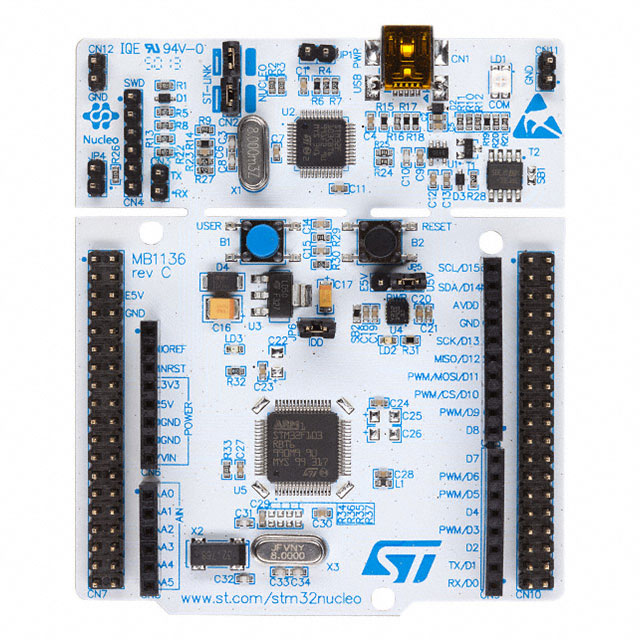
\includegraphics[width=0.85\linewidth]{pictures/nucleo_board.jpg}
    \caption{Микроконтролерна платка STM32L476RG Nucleo}
    %Да, ама не! Това е STM32F103
    \label{fig:nucleo}
\end{figure}
\FloatBarrier
Микроконтролерът се свързва с адресната магистрала, магистралата за данни и контролните сигнали на РОБКО 01. Това му позволява да чете и пише в регистрите на драйверната платка. Софтуерът на микроконтролера се разглежда подробно в глава \ref{firmware_chapter}. Основната му функция е да определя какви стойности да записва в регистрите на драйверната платка на РОБКО 01 за да бъдат изпълнени желаните движения.
\subsection{Основна платка и адаптери}
В рамките на настоящата разработка са проектирани и изработени три печатни платки. Две от тях са пасивни адаптери за специфичните конектори на РОБКО 01. Печатната платка означена на фигура \ref{fig:system} като "Основна платка" служи за централен възел на системата - свързва отделните модули един към друг. Също така предоставя визуална индикация за състоянието на моторите, възможност за настройка и петволтово захранване. Проектираните печатни платки се разглеждат подробно в глава \ref{boards_chapter}.
\subsection{USB/UART модул}
Комуникацията между сървърният компютър и микроконтролера се извършва по серийна UART връзка. Скоростта е 115200 бода, изпращат се осембитови думи с по един допълнителен бит за проверка по четност и предаването на данни се завършва с един стоп бит. Битът за проверка по четност е единица, когато в осемте бита на предаваната дума има четен брой единици. Връзката между микроконтролера и компютъра преминава през USB/UART адаптерна платка, показана на фигура \ref{fig:usb_uart}. Сървърният софтуер достъпва USB/UART модула като виртуален сериен порт, свързан по USB връзка.
\begin{figure}[!htb]
    \centering
    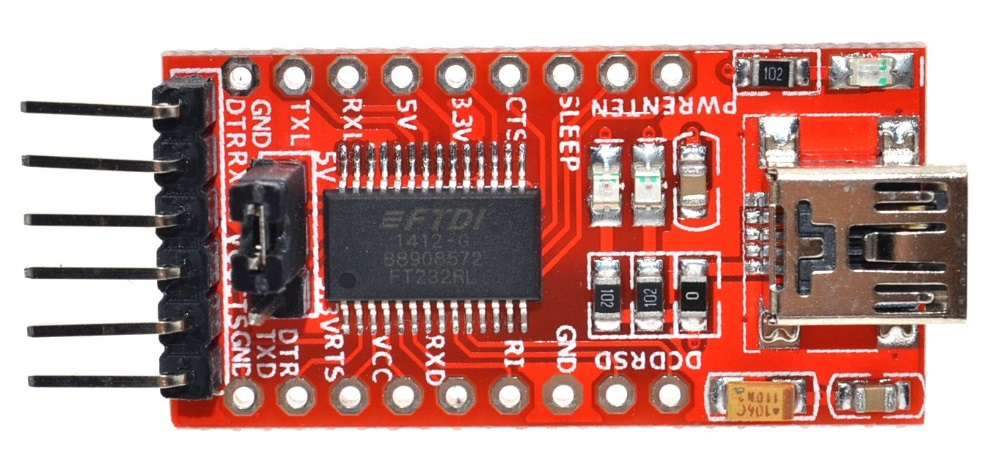
\includegraphics[width=0.75\linewidth]{pictures/USB_to_UART.jpg}
    \caption{USB/UART адаптерна платка}
    \label{fig:usb_uart}
\end{figure}
\FloatBarrier
\subsection{Компютри и софтуер за отдалечено управление}
Отдалеченото управление през Интернет се реализира чрез две програми - клиент и сървър. Клиентската програма чете текстови команди, въвеждани от потребителя в команден ред и ги изпраща през TCP сокет към сървърната програма. На сървъра се съхраняват файлове, съдържащи предварително въведени поредици от команди. Сървърната програма препраща получените команди към микроконтролера или прочита файл и изпраща записаните в него команди. Двете програми и форматът на командите се описват в глава \ref{network_chapter}.\\
\indent{}
За реализацията на проекта един и същи компютър е използван и като клиент, и като сървър. Клиентската програма се изпълнява на виртуална машина Ubuntu Server. Употребата на виртуална машина позволява клиентската и сървърната програма да използват различни IP адреси, което е наложително за тестване на мрежовата свързаност.\\
\indent{}
При имплементация на подобна система в промишлени условия сървърният компютър вероятно ще бъде индустриален, а клиентският - обикновен персонален компютър. Индустриалните компютри се отличават с по-високи изисквания за издръжливост на температура, прах, механични вибрации и удари, електромагнитни смущения и влага. Често разполагат със специализирани конектори и са предназначени за монтаж в табла, на стени или в шкафове.
%източник?
\subsection{Джойстици}
\label{joysticks}
Ръчното управление на робота се осъществява посредством два джойстика, показани на фигура \ref{fig:joysticks}. Разполагат с по два бутона и една дръжка. Джойстиците са произведени като периферни устройства за Правец 8\cite{joystick_pravets} и са директно копие на джойстик A2M2002, произвеждан от Apple.\cite{joystick_apple} Движението на дръжката завърта два потенциометъра. Измерването на съпротивлението им се е извършвало с помощта на таймер 558, свързан като чакащ мултивибратор. Продължителността на генерираните от таймера импулси е пропорционална на съпротивлението и съответно на позицията на дръжката на джойстика.
\cite{joystick_explained}\\
\indent{}
\begin{figure}[!htb]
    \centering
    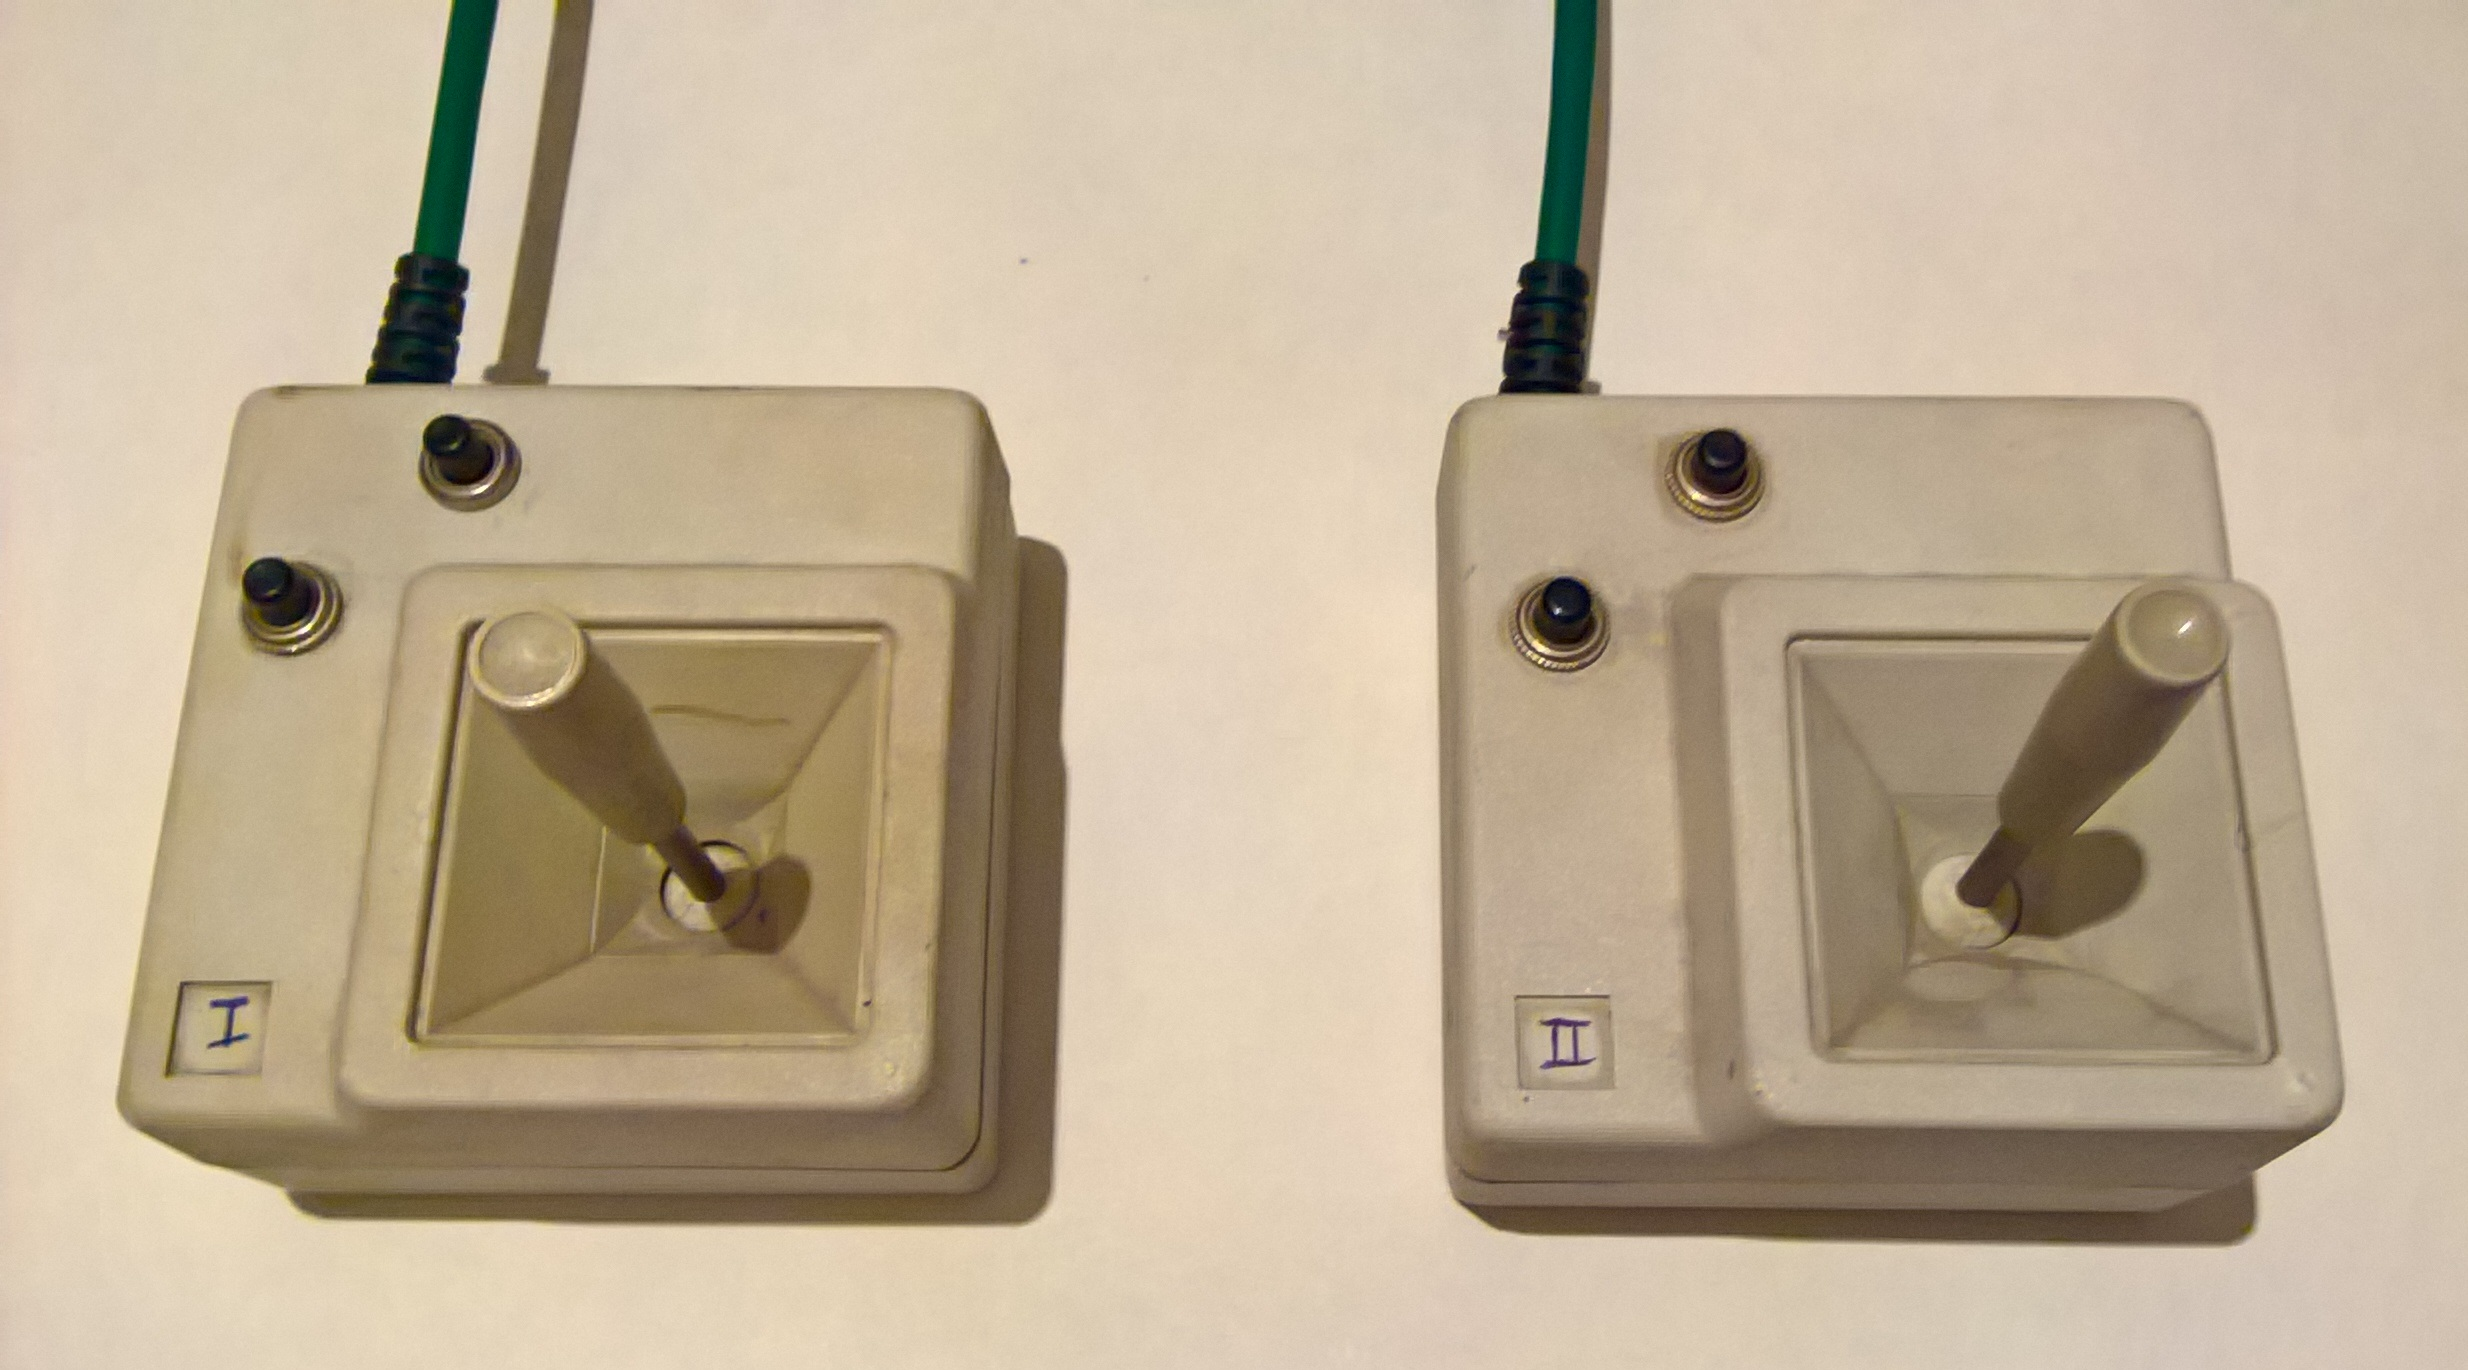
\includegraphics[width=\linewidth]{pictures/joysticks.jpg}
    \caption{Модифицирани джойстици за Правец 8}
    \label{fig:joysticks}
\end{figure}
За да се използват в настоящата разработка двата джойстика са модифицирани. Оригиналните им кабели са заменени с UTP Cat 5 кабели с накрайници RJ45. Неизползваните изводи на потенциометрите са свързани към захранващото напрежение, образувайки делител на напрежение. На следващата страница е показана принципната електрическа схема на джойстиците след извършените модификации. Първите два пина се използват за засичане на джойстиците от микроконтролера. Когато и двата джойстика са свързани към основната платка, през тези окъсени пинове се изгражда връзка между пин PC7 на микроконтролера и 3,3V захранване.\\
\indent{}
Първият джойстик се свързва към конектор RJ1 на основната платка, а вторият към RJ2 (виж точка \ref{manual_cntrl_section}). За горна страна се приема страната, от която излиза кабелът. В таблица \ref{tab:joysticks} се описва кой джойстик се използва за управлението на какви движения на РОБКО 01.
\begin{table}[!th]
    \centering
    \begin{tabular}{|c|c|c|}
        \hline
        Джойстик & Позиция/натиснат бутон & Движение на РОБКО 01\\
        \hline
        \multirow{6}{*}{Първи} & дръжка наляво & щипка - въртене наляво\\
        & дръжка надясно & щипка - въртене надясно\\
        \cline{2-3}
        & дръжка нагоре & повдигане лакът\\
        & дръжка надолу & сваляне лакът\\
        \cline{2-3}
        & горен бутон & щипка - завъртане нагоре\\
        & долен бутон & щипка - завъртане надолу\\
        \hline
        \multirow{6}{*}{Втори} & дръжка наляво & основа - въртене наляво\\
        & дръжка надясно & основа - въртене надясно\\
        \cline{2-3}
        & дръжка нагоре & рамо назад\\
        & дръжка надолу & рамо напред\\
        \cline{2-3}
        & горен бутон & щипка - стискане\\
        & долен бутон & щипка - отпускане\\
        \hline
    \end{tabular}
    \caption{Съответствия между джойстици и движения на РОБКО 01}
    \label{tab:joysticks}
\end{table}
\FloatBarrier
\includepdf[pages={6},angle=90]{documents/schematic_bw.pdf}
\subsection{Захранване}
Системата се захранва от 12-волтово импулсно захранване\footnote{с изключение на двата компютъра и USB/UART конверторната платка, която се захранва от сървърния компютър, виж фиг. \ref{fig:system}}, показано на фигура \ref{fig:psu}. Максималният изходен ток на захранването е 10A, максималната мощност е 120W. Според спецификациите на импулсното захранване входното му напрежение е в обхвата от 110V до 220V, но функционира правилно и при входно напрежение 230V.
\begin{figure}[!htb]
    \centering
    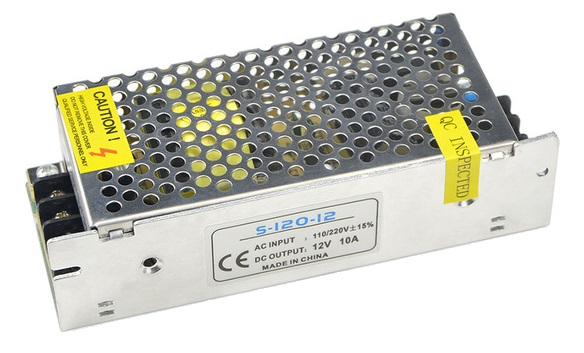
\includegraphics[width=0.8\linewidth]{pictures/PSU.jpg}
    \caption{Захранващ източник}
    \label{fig:psu}
\end{figure}